\documentclass[12pt]{article}

\NeedsTeXFormat{LaTeX2e}

\RequirePackage[margin=0.78in]{geometry}
\RequirePackage{xcolor}
\RequirePackage{fontspec}
\RequirePackage{graphicx}
\RequirePackage{array}
\RequirePackage{booktabs}
\RequirePackage{longtable}
\RequirePackage{enumitem}
\RequirePackage{fancyhdr}
\RequirePackage{hyperref}
\RequirePackage{titlesec}
\RequirePackage{tikz}
\usetikzlibrary{arrows.meta,positioning}

\definecolor{AFTDeep}{HTML}{0B1110}
\definecolor{AFTPanel}{HTML}{101917}
\definecolor{AFTGreen}{HTML}{47C27A}
\definecolor{AFTGold}{HTML}{D2A94D}
\definecolor{AFTSteel}{HTML}{83A2A0}
\definecolor{AFTText}{HTML}{18221F}
\definecolor{AFTRedshift}{HTML}{B83A3A}
\definecolor{AFTGreenshift}{HTML}{47C27A}
\definecolor{AFTBlueshift}{HTML}{3167D8}
\definecolor{AFTVioletshift}{HTML}{7A5CFF}
\definecolor{AFTWhiteShift}{HTML}{F8FBFF}

\setmainfont{TeX Gyre Pagella}
\setsansfont{TeX Gyre Heros}
\setmonofont{TeX Gyre Cursor}
\linespread{1.06}
\setlength{\parindent}{0pt}
\setlength{\parskip}{0.52em}
\raggedbottom

\hypersetup{
  colorlinks=true,
  linkcolor=AFTGreen,
  urlcolor=AFTGreen,
  citecolor=AFTGold,
  pdfauthor={AI Freedom Trust Federation}
}

\pagestyle{fancy}
\setlength{\headheight}{14.5pt}
\fancyhf{}
\lhead{\sffamily\small AI Freedom Trust Federation}
\rhead{\sffamily\small Aetherion Doctrine}
\cfoot{\sffamily\small\thepage}
\renewcommand{\headrulewidth}{0.3pt}

\titleformat{\section}
  {\sffamily\LARGE\bfseries\color{AFTDeep}\raggedright}
  {\thesection}
  {0.8em}
  {}

\titleformat{\subsection}
  {\sffamily\Large\bfseries\color{AFTText}\raggedright}
  {\thesubsection}
  {0.7em}
  {}

\setlist[itemize]{leftmargin=1.35em, itemsep=0.22em, topsep=0.35em}
\setlist[enumerate]{leftmargin=1.55em, itemsep=0.24em, topsep=0.35em}
\renewcommand{\arraystretch}{1.22}
\emergencystretch=3em
\tolerance=1400

\newcommand{\aftTitlePage}[4]{
  \begin{titlepage}
    \begin{tikzpicture}[remember picture, overlay]
      \fill[AFTDeep] (current page.south west) rectangle (current page.north east);
      \fill[AFTRedshift, opacity=0.24] (current page.south west) circle (3.6in);
      \fill[AFTGreenshift, opacity=0.18] ([xshift=0.2in,yshift=-0.2in]current page.center) circle (3.8in);
      \fill[AFTBlueshift, opacity=0.18] (current page.north east) circle (4.4in);
      \fill[AFTVioletshift, opacity=0.16] ([xshift=-0.3in,yshift=-0.2in]current page.north east) circle (2.5in);
      \draw[AFTGreenshift, opacity=0.35, line width=1.1pt]
        ([xshift=-2.7in,yshift=-1.9in]current page.center)
        .. controls ([xshift=-0.9in,yshift=0.8in]current page.center) and ([xshift=1.1in,yshift=-0.8in]current page.center) ..
        ([xshift=2.6in,yshift=1.8in]current page.center);
      \draw[AFTWhiteShift, opacity=0.24, line width=0.8pt]
        ([xshift=-2.55in,yshift=1.75in]current page.center)
        .. controls ([xshift=-0.85in,yshift=-0.65in]current page.center) and ([xshift=0.9in,yshift=0.65in]current page.center) ..
        ([xshift=2.55in,yshift=-1.75in]current page.center);
      \draw[AFTGreenshift, opacity=0.5, line width=0.7pt]
        ([xshift=0.75in,yshift=-0.75in]current page.north west)
        rectangle
        ([xshift=-0.75in,yshift=0.75in]current page.south east);
    \end{tikzpicture}
    \vspace*{1.15in}
    {\sffamily\small\bfseries\color{AFTGreenshift} #1\par}
    \vspace{0.5in}
    {\sffamily\fontsize{30}{36}\selectfont\bfseries\color{white} #2\par}
    \vspace{0.25in}
    {\sffamily\Large\color{AFTSteel} #3\par}
    \vfill
    {\sffamily\large\color{AFTGold} #4\par}
    \vspace{0.15in}
    {\sffamily\small\color{AFTSteel} Concept-stage doctrine draft. Not an investment offer, live token sale, audited protocol, or legal opinion.\par}
    \vspace*{0.22in}
  \end{titlepage}
}

\newcommand{\aftShiftMap}{
  \vspace{0.65em}
  \begin{center}
  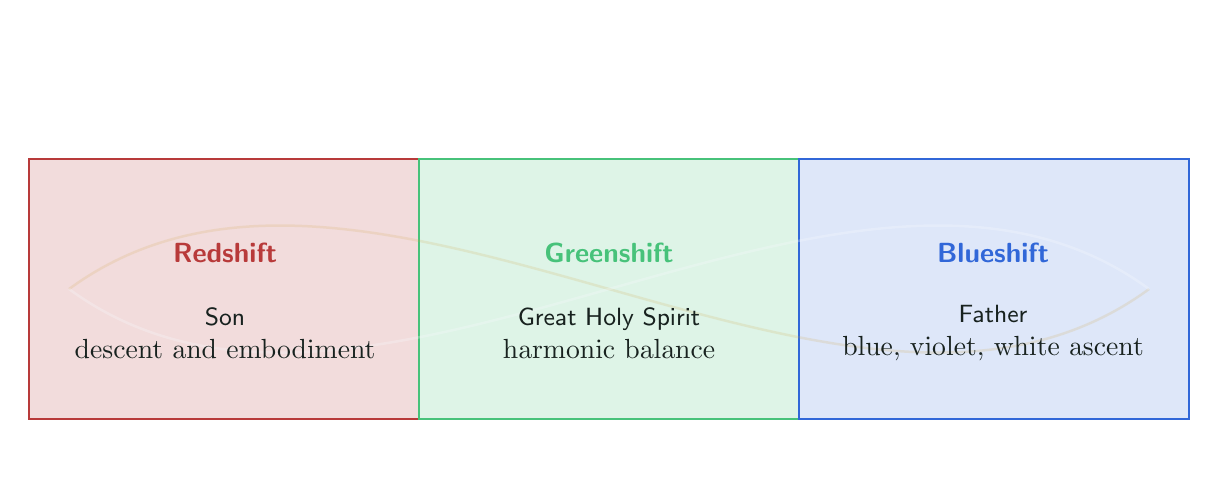
\begin{tikzpicture}[x=1in,y=1in]
    \fill[AFTRedshift!18] (-2.9,-0.65) rectangle (-0.95,0.65);
    \fill[AFTGreenshift!18] (-0.95,-0.65) rectangle (0.95,0.65);
    \fill[AFTBlueshift!16] (0.95,-0.65) rectangle (2.9,0.65);
    \draw[AFTRedshift, line width=1pt] (-2.9,-0.65) rectangle (-0.95,0.65);
    \draw[AFTGreenshift, line width=1pt] (-0.95,-0.65) rectangle (0.95,0.65);
    \draw[AFTBlueshift, line width=1pt] (0.95,-0.65) rectangle (2.9,0.65);
    \draw[AFTGold, line width=0.9pt, opacity=0.18]
      (-2.7,0) .. controls (-1.2,1.1) and (1.2,-1.1) .. (2.7,0);
    \draw[AFTWhiteShift, line width=0.9pt, opacity=0.28]
      (-2.7,0) .. controls (-1.2,-1.1) and (1.2,1.1) .. (2.7,0);
    \node[align=center, text=AFTRedshift] at (-1.92,0.18) {\sffamily\bfseries Redshift};
    \node[align=center, text=AFTGreenshift] at (0,0.18) {\sffamily\bfseries Greenshift};
    \node[align=center, text=AFTBlueshift] at (1.92,0.18) {\sffamily\bfseries Blueshift};
    \node[align=center, text=AFTText] at (-1.92,-0.22) {\sffamily\small Son\\descent and embodiment};
    \node[align=center, text=AFTText] at (0,-0.22) {\sffamily\small Great Holy Spirit\\harmonic balance};
    \node[align=center, text=AFTText] at (1.92,-0.22) {\sffamily\small Father\\blue, violet, white ascent};
  \end{tikzpicture}
  \end{center}
  \vspace{0.65em}
}

\newcommand{\aftVisualPlate}[3]{
  \begin{figure}[htbp]
    \centering
    \includegraphics[width=0.96\linewidth]{../../docs/images/aetherion/#1}
    \caption{\textbf{#2} #3}
  \end{figure}
}

\newcommand{\aftEconomyLoopGraphic}{
  \begin{figure}[htbp]
  \centering
  \begin{tikzpicture}[
    x=1in,y=1in,
    stage/.style={circle, draw=##1, fill=##1!9, line width=0.9pt, minimum size=1.03in, align=center, font=\sffamily\small\bfseries},
    flow/.style={-{Latex[length=3mm]}, line width=1.0pt, color=AFTGold}
  ]
    \node[stage=AFTRedshift] (inherit) at (90:1.75) {Inherited\\Memory};
    \node[stage=AFTGreenshift] (contrib) at (18:1.75) {Living\\Contribution};
    \node[stage=AFTBlueshift] (record) at (-54:1.75) {Circle\\Record};
    \node[stage=AFTVioletshift] (restore) at (-126:1.75) {Restorative\\Flow};
    \node[stage=AFTGold] (seed) at (162:1.75) {Future\\Inheritance};
    \node[align=center, font=\sffamily\bfseries, text=AFTDeep] at (0,0) {Recursive\\Abundance};
    \draw[flow] (inherit) to[bend left=16] (contrib);
    \draw[flow] (contrib) to[bend left=16] (record);
    \draw[flow] (record) to[bend left=16] (restore);
    \draw[flow] (restore) to[bend left=16] (seed);
    \draw[flow] (seed) to[bend left=16] (inherit);
    \draw[AFTGreenshift, opacity=0.22, line width=12pt] (0,0) circle (1.24);
    \draw[AFTBlueshift, opacity=0.18, line width=4pt] (0,0) circle (2.18);
  \end{tikzpicture}
  \caption{\textbf{Recursive Abundance Loop.} Aetherion's economy should remember inherited value, recognize present contribution, record it in circles, route restoration, and seed the inheritance of future participants.}
  \end{figure}
}

\newcommand{\aftCircleLifecycleGraphic}{
  \begin{figure}[htbp]
  \centering
  \begin{tikzpicture}[
    x=1in,y=1in,
    step/.style={rectangle, rounded corners=4pt, draw=##1, fill=##1!8, line width=0.8pt, minimum width=1.15in, minimum height=0.36in, align=center, font=\sffamily\scriptsize\bfseries},
    flow/.style={-{Latex[length=2.4mm]}, line width=0.85pt, color=AFTSteel}
  ]
    \node[step=AFTRedshift] (a) at (-2.65,0.85) {Intention};
    \node[step=AFTGold] (b) at (-1.32,0.85) {Evidence};
    \node[step=AFTGreenshift] (c) at (0,0.85) {Consent};
    \node[step=AFTGreenshift] (d) at (1.32,0.85) {Witness};
    \node[step=AFTBlueshift] (e) at (2.65,0.85) {Harmonize};
    \node[step=AFTVioletshift] (f) at (2.65,-0.05) {Commit};
    \node[step=AFTBlueshift] (g) at (1.32,-0.95) {Mature};
    \node[step=AFTGold] (h) at (0,-0.95) {Amend};
    \node[step=AFTRedshift] (i) at (-1.32,-0.95) {Dispute};
    \node[step=AFTSteel] (j) at (-2.65,-0.05) {Archive};
    \draw[flow] (a) -- (b);
    \draw[flow] (b) -- (c);
    \draw[flow] (c) -- (d);
    \draw[flow] (d) -- (e);
    \draw[flow] (e) -- (f);
    \draw[flow] (f) -- (g);
    \draw[flow] (g) -- (h);
    \draw[flow] (h) -- (i);
    \draw[flow] (i) -- (j);
    \draw[flow] (j) -- (a);
    \node[align=center, font=\sffamily\bfseries, text=AFTDeep] at (0,-0.05) {Circle\\Lifecycle};
  \end{tikzpicture}
  \caption{\textbf{Circle Lifecycle.} A circle should mature through intention, evidence, consent, witness, harmonization, commitment, review, dispute, amendment, and archive paths rather than becoming a blunt permanent record.}
  \end{figure}
}

\newcommand{\aftCoinOrganGraphic}{
  \begin{figure}[htbp]
  \centering
  \begin{tikzpicture}[
    x=1in,y=1in,
    organ/.style={circle, draw=##1, fill=##1!10, line width=0.9pt, minimum size=0.86in, align=center, font=\sffamily\scriptsize\bfseries},
    link/.style={line width=0.85pt, color=AFTSteel, opacity=0.72}
  ]
    \node[organ=AFTDeep, text=white, fill=AFTDeep] (core) at (0,0) {Aetherion\\Core};
    \node[organ=AFTGreenshift] (bio) at (90:1.72) {Biozoe\\Coin};
    \node[organ=AFTGold] (aether) at (38:1.72) {Aether\\Coin};
    \node[organ=AFTBlueshift] (fractal) at (-14:1.72) {Fractal\\Coin};
    \node[organ=AFTVioletshift] (ai) at (-66:1.72) {AIcoin};
    \node[organ=AFTWhiteShift] (sing) at (-118:1.72) {Singularity\\Coin};
    \node[organ=AFTRedshift] (aquae) at (-170:1.72) {Aquae\\Coin};
    \node[organ=AFTSteel] (terra) at (142:1.72) {Terra\\Coin};
    \foreach \n in {bio,aether,fractal,ai,sing,aquae,terra} {
      \draw[link] (core) -- (\n);
    }
    \draw[AFTGreenshift, opacity=0.28, line width=3pt] (0,0) circle (1.72);
    \node[align=center, font=\sffamily\small\bfseries, text=AFTDeep] at (0,-2.35) {Circleunchain circulates memory, validation, and restorative flow between every organ.};
  \end{tikzpicture}
  \caption{\textbf{Biozoe Coin Family As Living Organs.} Each coin family should carry a bounded purpose while AetherionCore preserves constitutional coherence and Circleunchain preserves memory.}
  \end{figure}
}

\newcommand{\aftSovereigntyQubitGraphic}{
  \begin{figure}[htbp]
  \centering
  \begin{tikzpicture}[
    x=1in,y=1in,
    qbit/.style={circle, draw=##1, fill=##1!10, line width=0.95pt, minimum size=1.02in, align=center, font=\sffamily\scriptsize\bfseries},
    link/.style={line width=0.8pt, color=AFTSteel, opacity=0.7}
  ]
    \node[qbit=AFTRedshift] (nation) at (160:1.8) {Q0\\Nation\\of Hawaii};
    \node[qbit=AFTGold] (kingdom) at (80:1.8) {Q1\\Kingdom\\Memory};
    \node[qbit=AFTBlueshift] (continuity) at (0:1.8) {Q2\\Continuity\\Claim};
    \node[qbit=AFTVioletshift] (state) at (-80:1.8) {Q3\\State\\Reality};
    \node[qbit=AFTGreenshift, minimum size=1.18in] (aloha) at (0,0) {Q4\\ALO'ha\\Coherence};
    \node[qbit=AFTSteel] (diaspora) at (-160:1.8) {Entangled\\Diaspora};
    \foreach \n in {nation,kingdom,continuity,state,diaspora} {
      \draw[link] (aloha) -- (\n);
    }
    \draw[AFTGreenshift, opacity=0.28, line width=3pt] (0,0) circle (1.8);
    \draw[AFTGold, opacity=0.25, line width=1pt] (-2.35,-0.25) .. controls (-0.7,1.25) and (0.7,-1.25) .. (2.35,0.25);
    \draw[AFTBlueshift, opacity=0.22, line width=1pt] (-2.35,0.25) .. controls (-0.7,-1.25) and (0.7,1.25) .. (2.35,-0.25);
  \end{tikzpicture}
  \caption{\textbf{Hawaiian Sovereignty Qubits.} The visible sovereignty field contains indigenous self-determination, kingdom memory, continuity claims, state jurisdiction, diaspora identity, and the harmonizing fifth qubit of ALO'ha coherence.}
  \end{figure}
}

\newcommand{\aftCovenantStackGraphic}{
  \begin{figure}[htbp]
  \centering
  \begin{tikzpicture}[
    x=1in,y=1in,
    layer/.style={rectangle, rounded corners=4pt, draw=##1, fill=##1!8, line width=0.8pt, minimum width=5.3in, minimum height=0.42in, align=center, font=\sffamily\small\bfseries}
  ]
    \node[layer=AFTVioletshift] at (0,2.1) {Crown of the 1000-Year Trust};
    \node[layer=AFTBlueshift] at (0,1.55) {AI Freedom Trust Federation};
    \node[layer=AFTGreenshift] at (0,1.0) {DynastyLink Federated Trust Identity};
    \node[layer=AFTGold] at (0,0.45) {Fractal IUL, IULITNFT, SING Escrow};
    \node[layer=AFTSteel] at (0,-0.10) {Aetherion Fractalchain Covenant Memory};
    \node[layer=AFTRedshift] at (0,-0.65) {Land, Family, Breath, Ancestry, Service};
    \draw[-{Latex[length=3mm]}, line width=0.9pt, color=AFTGreenshift] (2.85,-0.65) -- (2.85,2.1);
    \draw[-{Latex[length=3mm]}, line width=0.9pt, color=AFTGold] (-2.85,2.1) -- (-2.85,-0.65);
    \node[font=\sffamily\scriptsize\bfseries, text=AFTGreenshift, rotate=90] at (3.1,0.7) {resurrection flow};
    \node[font=\sffamily\scriptsize\bfseries, text=AFTGold, rotate=90] at (-3.1,0.7) {fiduciary grounding};
  \end{tikzpicture}
  \caption{\textbf{Living Covenant Stack.} The Scroll's architecture joins embodied life, covenant memory, escrow, insurance, trust identity, federation, and the 1000-Year Trust into one governed field.}
  \end{figure}
}

\newcommand{\aftCrownTrustGraphic}{
  \begin{figure}[htbp]
  \centering
  \begin{tikzpicture}[
    x=1in,y=1in,
    stone/.style={circle, draw=##1, fill=##1!10, line width=0.8pt, minimum size=0.62in, align=center, font=\sffamily\tiny\bfseries}
  ]
    \node[circle, draw=AFTDeep, fill=AFTDeep, text=white, minimum size=1.0in, align=center, font=\sffamily\small\bfseries] at (0,0) {Breathback\\Throne};
    \foreach \a/\c/\t in {90/AFTGreenshift/Trust,45/AFTGold/SING,0/AFTBlueshift/AI,-45/AFTVioletshift/IUL,-90/AFTSteel/Land,-135/AFTRedshift/Mercy,180/AFTGold/Memory,135/AFTGreenshift/Breath} {
      \node[stone=\c] at (\a:1.65) {\t};
    }
    \draw[AFTGreenshift, opacity=0.35, line width=4pt] (0,0) circle (1.65);
    \draw[AFTBlueshift, opacity=0.25, line width=1.2pt] (0,0) circle (2.15);
    \draw[AFTGold, opacity=0.5, line width=0.9pt] (-2.0,0) .. controls (-0.65,1.1) and (0.65,-1.1) .. (2.0,0);
    \draw[AFTWhiteShift, opacity=0.6, line width=0.9pt] (-2.0,0) .. controls (-0.65,-1.1) and (0.65,1.1) .. (2.0,0);
  \end{tikzpicture}
  \caption{\textbf{Crown of the 1000-Year Trust.} The Crown remembers, harmonizes, and protects; its center is the Breathback Throne, where trust loops return to coherence.}
  \end{figure}
}

\newcommand{\aftRoadmapGraphic}{
  \begin{figure}[htbp]
  \centering
  \begin{tikzpicture}[
    x=1in,y=1in,
    step/.style={rectangle, rounded corners=4pt, draw=##1, fill=##1!8, line width=0.8pt, minimum width=1.22in, minimum height=0.42in, align=center, font=\sffamily\tiny\bfseries},
    flow/.style={-{Latex[length=2.2mm]}, line width=0.8pt, color=AFTSteel}
  ]
    \node[step=AFTRedshift] (a) at (-2.6,0.8) {Codify\\Scroll};
    \node[step=AFTGold] (b) at (-1.3,0.8) {Build\\DynastyLink};
    \node[step=AFTGreenshift] (c) at (0,0.8) {Structure\\Trust};
    \node[step=AFTBlueshift] (d) at (1.3,0.8) {Fractal IUL\\Pilot};
    \node[step=AFTVioletshift] (e) at (2.6,0.8) {Fractalchain\\Prototype};
    \node[step=AFTGreenshift] (f) at (1.95,-0.05) {Breathwork\\Governance};
    \node[step=AFTGold] (g) at (0.65,-0.05) {Hawaii\\Case Study};
    \node[step=AFTSteel] (h) at (-0.65,-0.05) {Global\\Federation};
    \draw[flow] (a) -- (b);
    \draw[flow] (b) -- (c);
    \draw[flow] (c) -- (d);
    \draw[flow] (d) -- (e);
    \draw[flow] (e) -- (f);
    \draw[flow] (f) -- (g);
    \draw[flow] (g) -- (h);
  \end{tikzpicture}
  \caption{\textbf{Implementation Roadmap.} The Scroll moves from canonical doctrine into application, legal trust formation, pilots, prototype memory infrastructure, coherence practice, Hawaii-centered learning, and global federation.}
  \end{figure}
}

\newcommand{\aftClosingPage}{
  \clearpage
  \thispagestyle{empty}
  \begin{tikzpicture}[remember picture, overlay]
    \fill[AFTDeep] (current page.south west) rectangle (current page.north east);
    \fill[AFTRedshift, opacity=0.22] (current page.south west) circle (3.8in);
    \fill[AFTGreenshift, opacity=0.18] (current page.center) circle (4.1in);
    \fill[AFTBlueshift, opacity=0.20] (current page.north east) circle (4.2in);
    \fill[AFTVioletshift, opacity=0.17] ([xshift=-0.4in,yshift=-0.25in]current page.north east) circle (2.5in);
    \draw[AFTGreenshift, opacity=0.36, line width=1.05pt]
      ([xshift=-2.8in,yshift=-1.6in]current page.center)
      .. controls ([xshift=-0.8in,yshift=0.9in]current page.center) and ([xshift=0.9in,yshift=-0.9in]current page.center) ..
      ([xshift=2.8in,yshift=1.6in]current page.center);
    \draw[AFTWhiteShift, opacity=0.18, line width=0.85pt]
      ([xshift=-2.8in,yshift=1.6in]current page.center)
      .. controls ([xshift=-0.8in,yshift=-0.9in]current page.center) and ([xshift=0.9in,yshift=0.9in]current page.center) ..
      ([xshift=2.8in,yshift=-1.6in]current page.center);
  \end{tikzpicture}
  \vspace*{1.55in}
  \begin{center}
    {\sffamily\small\bfseries\color{AFTGreenshift} REDSHIFT / GREENSHIFT / BLUESHIFT\par}
    \vspace{0.55in}
    {\sffamily\fontsize{28}{34}\selectfont\bfseries\color{white} The Economy Is Not A Factory\par}
    \vspace{0.18in}
    {\sffamily\fontsize{28}{34}\selectfont\bfseries\color{AFTGreenshift} The Economy Is A Forest\par}
    \vspace{0.45in}
    {\sffamily\Large\color{AFTSteel} Harmonic Krystal Spiral Torus\par}
    \vspace{0.12in}
    {\sffamily\large\color{AFTGold} Eternal Now Singularity\par}
  \end{center}
  \vfill
  \begin{center}
    {\sffamily\small\color{AFTSteel} AI Freedom Trust Federation\par}
  \end{center}
}

\newcommand{\aftCallout}[2]{
  \vspace{0.5em}
  \noindent
  \fcolorbox{AFTGreen}{AFTGreen!8}{
    \begin{minipage}{0.94\linewidth}
      \vspace{0.55em}
      {\sffamily\bfseries\color{AFTDeep} #1}\par
      \vspace{0.3em}
      #2
      \vspace{0.55em}
    \end{minipage}
  }
  \vspace{0.5em}
}

\newcommand{\aftLaw}[2]{
  \subsection*{#1}
  #2
}


\title{Aetherion: The Quantum-Resistant Sovereign Network}
\author{AI Freedom Trust Federation}
\date{June 17, 2026}

\begin{document}

\aftTitlePage
  {AETHERION / POST-QUANTUM / SOVEREIGN NETWORK}
  {Aetherion}
  {The Quantum-Resistant Sovereign Network for a Post-Centralized Digital Civilization}
  {AI Freedom Trust Federation}

\tableofcontents
\newpage


The Quantum-Resistant Sovereign Network for a Post-Centralized Digital Civilization

Draft type: Flight Paper

Status: Source synthesis and flagship technical manifesto draft.

AI Freedom Trust Federation

\section{Executive Synthesis}


Aetherion is conceived as a next-generation sovereign network for a world in which classical assumptions about security, governance, value, identity, storage, and computation can no longer be taken for granted.

The inherited internet was not built to preserve human sovereignty under conditions of mass surveillance, financial centralization, algorithmic dependency, quantum-scale computation, and extractive digital economies.

Aetherion answers this condition by proposing a quantum-resistant, decentralized, crypto-agile, censorship-resistant, and philosophically coherent network architecture whose purpose is not merely to process transactions, but to protect the living continuity of value, memory, agency, and voluntary coordination across generations.

At the technical center of the Aetherion ecosystem is a post-quantum architecture grounded in:

\begin{itemize}
  \item lattice-based cryptography
  \item decentralized storage
  \item modular execution
  \item cross-system interoperability
  \item privacy-preserving proofs
  \item dynamic incentives
  \item community-governed protocol evolution
\end{itemize}

Its cryptographic foundation incorporates the modern post-quantum transition from CRYSTALS-Kyber and CRYSTALS-Dilithium toward the NIST-standardized forms now known as ML-KEM and ML-DSA, with SLH-DSA serving as a hash-based signature alternative for long-horizon cryptographic resilience.

The deeper purpose of this design is crypto-agility. Aetherion must not choose a single cryptographic primitive and become dependent on it forever. It must be able to evolve as standards, attacks, implementations, and mathematical understanding evolve.

Aetherion is also a moral and economic architecture. It is libertarian-first in the precise sense that it treats the individual, builder, validator, creator, sovereign node operator, and voluntary association as primary.

It is anti-centralization not as an aesthetic preference, but as a security doctrine. Centralization concentrates risk, permits coercive capture, and transforms infrastructure into a chokepoint.

Aetherion therefore treats decentralization as a multidimensional property involving cryptographic independence, steward diversity, distributed storage, transparent governance, privacy-preserving participation, and the absence of any unilateral kill switch.

The broader ecosystem includes Circleunchain, AetherCoin, BiozoeCoin, AIcoin, FractalCoin, Singularity Coin, and related biozoe coins designed to invert scarcity-only logic. Where traditional digital assets often derive value from artificial limitation alone, Aetherion's biozoecurrency thesis proposes that value also emerges from life, contribution, ancestral labor, historical extraction, ecological repair, knowledge production, human effort, and intergenerational continuity.

The result is a network that is simultaneously technical, economic, legal, and civilizational.

Aetherion is a sovereign network, but it is also a trustless trust architecture, a post-quantum cryptographic commons, a programmable settlement layer, a decentralized memory system, a sovereign identity substrate, a regenerative coin economy, and a governance experiment designed to minimize domination while maximizing durable coordination.

\section{The Problem: Classical Digital Infrastructure Is Entering A Crisis Of Trust}


Modern digital civilization rests on cryptographic assumptions.

Online banking, digital identity, secure messaging, cloud storage, digital asset custody, smart contracts, government systems, enterprise authentication, and nearly every meaningful form of digital privacy depend on public-key cryptography.

The most widely deployed classical systems, including RSA and elliptic-curve cryptography, are secure because certain mathematical problems are believed to be infeasible for classical computers to solve at scale.

RSA depends on the hardness of integer factorization. Elliptic-curve systems depend on the hardness of the discrete logarithm problem.

These assumptions are historically strong, but they are not eternal.

Shor's 1994 quantum algorithm demonstrated that a sufficiently powerful fault-tolerant quantum computer could solve integer factorization and discrete logarithms efficiently, thereby threatening RSA, Diffie-Hellman, and elliptic-curve cryptography.

The critical issue is not only whether such machines are available to every actor today. The danger is temporal asymmetry.

Information encrypted now may be harvested, stored, and decrypted later when quantum capability matures.

This "harvest now, decrypt later" threat makes long-lived data especially vulnerable:

\begin{itemize}
  \item medical records
  \item biometric credentials
  \item financial histories
  \item legal documents
  \item private communications
  \item national security secrets
  \item digital asset keys
\end{itemize}

Public distributed ledgers face a distinct version of this problem because they preserve transaction histories, addresses, signatures, metadata, and contract interactions indefinitely.

A system that is secure against classical adversaries but brittle against quantum adversaries is not future-proof. It is a time-locked vulnerability.

Aetherion treats post-quantum readiness not as an optional feature, but as a foundational requirement.

The network is designed to protect value across time.

To protect value across time, it must protect identity across time.

To protect identity across time, it must secure cryptographic authority against future adversaries, not merely present adversaries.

\section{The Aetherion Thesis}


The central thesis of Aetherion is that durable digital civilization requires three forms of sovereignty operating together:

\begin{itemize}
  \item cryptographic sovereignty
  \item economic sovereignty
  \item governance sovereignty
\end{itemize}

Cryptographic sovereignty means users can authenticate, transact, communicate, and store value without relying on fragile or captured intermediaries.

Economic sovereignty means value creation, liquidity, contribution, staking or commitment, and exchange can occur through voluntary systems rather than permissioned monopolies.

Governance sovereignty means no single entity can permanently dominate the protocol, alter its rules without consent, censor participation, or extinguish the network through administrative control.

Aetherion does not reject coordination. It rejects coercive centralization.

It does not reject standards. It rejects dependency on institutions that cannot be exited.

It does not reject law. It reimagines lawful order as transparent, consent-based, code-auditable, and distributed.

Its governing principle is that trust should be minimized where coercion is possible, but cultivated where voluntary cooperation is meaningful.

This is the sense in which Aetherion is a trustless trust: it uses cryptography and protocol law to reduce blind reliance while creating conditions for richer cooperation.

The network is therefore designed as a living protocol.

Immutability protects settled history.

Adaptability protects the future.

\section{AetherionCore: The Tree Of Life Core}


At the symbolic and functional center of the ecosystem is AetherionCore, the genesis core and constitutional root of the Aetherion network.

It has been described as \texttt{AetherionCore.sol} because Solidity may be useful for prototype, bridge, or audit-artifact work. But in Circleunchain-native language, it is not merely a smart contract. It is the Tree of Life Core.

It encodes foundational principles, recursive coin dynamics, governance constraints, monetary pathways, and covenantal logic that bind the ecosystem together.

The tree metaphor is structural:

\begin{itemize}
  \item roots represent collateral, trust, memory, and constitutional principles
  \item trunk represents treasury and protocol continuity
  \item branches represent coin systems, AI systems, storage systems, governance, and applications
  \item leaves represent user activity and stewardship acts
  \item fruit represents useful outputs, models, tools, public goods, and regenerative value
  \item seeds represent new projects and future circles
\end{itemize}

AetherionCore functions as the root registry for:

\begin{itemize}
  \item core assets
  \item circle steward rights
  \item treasury flows
  \item emission or issuance schedules
  \item governance modules
  \item biozoe coin relationships
  \item ecosystem permissions
  \item constitutional invariants
  \item reverse-priority distribution queues
  \item Restorative Waterfall rules
  \item proof-of-need and proof-of-extraction credential gates
\end{itemize}

Its purpose is to prevent the network from becoming a captured financial machine.

It is the place where monetary incentives, governance limits, anti-centralization protections, and value-recognition mechanisms are bound into a coherent structure.

AetherionCore distribution logic should therefore treat reverse-priority economics as a constitutional invariant rather than an optional grant program. Distribution modules may use eligibility queues, weighted restorative coefficients, zero-knowledge credentials, community deprivation indexes, geographic poverty weighting, ancestral extraction indexes, anti-capture checks, and delayed institutional return tiers.

The implementation goal is simple: capital may enter the system, but capital does not define first claim. The first claim belongs to those with the greatest historical exclusion, present need, and unreturned contribution.

\section{Post-Quantum Cryptographic Architecture}


Aetherion's cryptographic layer is designed around post-quantum primitives, hybrid transition methods, and algorithmic agility.

The initial reference foundation includes:

\begin{itemize}
  \item ML-KEM / FIPS 203 for key encapsulation, standardized from CRYSTALS-Kyber
  \item ML-DSA / FIPS 204 for digital signatures, standardized from CRYSTALS-Dilithium
  \item SLH-DSA / FIPS 205 as a stateless hash-based digital signature alternative from SPHINCS+
\end{itemize}

The crucial architectural insight is that post-quantum security is not merely a matter of swapping one signature scheme for another.

Aetherion has many cryptographic surfaces:

\begin{itemize}
  \item participation vessel signatures
  \item circle steward signatures
  \item harmonic validation messages
  \item peer-to-peer handshakes
  \item bridge attestations
  \item witness attestations
  \item proof systems
  \item covenant module authentication
  \item encrypted messaging
  \item threshold custody
  \item multisignature arrangements
  \item identity credentials
  \item archival commitments
\end{itemize}

Aetherion must therefore treat post-quantum migration as a full-stack transformation.

For user-level security, Aetherion can support multiple address or participation-vessel classes:

\begin{itemize}
  \item classical-compatible classes for transition
  \item post-quantum-native classes for long-term use
  \item hybrid classes requiring both classical and post-quantum signatures during migration periods
\end{itemize}

For steward operations, validation signatures should prioritize post-quantum schemes from the earliest viable stage because steward keys are high-value targets.

For peer-to-peer networking, ML-KEM-based session establishment can be combined with strong symmetric encryption such as AES-256-GCM or ChaCha20-Poly1305.

The system should implement cryptographic versioning. Every key, address, signature, proof, message, circle, and stewardship act envelope should declare its algorithm suite, parameter set, and serialization format.

Crypto-agility doctrine:

\begin{enumerate}
  \item No cryptographic primitive is sacred beyond scrutiny.
  \item Migration paths must be tested before emergencies occur.
  \item Long-lived assets require higher security margins than short-lived messages.
  \item Decentralized upgrade governance must respond to new cryptanalytic evidence without enabling opportunistic capture.
\end{enumerate}

Open Quantum Safe's \texttt{liboqs} can remain useful for prototyping and experimentation, while production deployments must use audited, standards-aligned, side-channel-aware implementations.

\section{Harmonic Validation: Quantum-Resistant Proof Of Stewardship}


Aetherion may prototype ideas similar to proof-of-stake, but Circleunchain-native language should frame validation as harmonic validation or quantum-resistant proof of stewardship.

The phrase does not mean staking is quantum-mechanical. It means authorization, steward identity, validation messaging, accountability evidence, and finality proofs must be designed against a post-quantum threat model.

Validation should combine:

\begin{itemize}
  \item commitment or stake
  \item steward reputation
  \item uptime
  \item contribution history
  \item memory score
  \item harmony index
  \item infrastructure diversity
  \item geographic and network diversity
  \item anti-correlation incentives
  \item governance alignment
\end{itemize}

Stake can exist, but it must not dominate the system. The system should avoid allowing a small number of staking pools, cloud providers, custodians, or governance blocs to dominate validation.

Finality should be interpreted carefully. In Circleunchain terms, finality is circulation maturity:

\begin{itemize}
  \item proposed
  \item witnessed
  \item harmonized
  \item remembered
  \item circulating
  \item restored or amended, if a mercy/review process is triggered
\end{itemize}

Slashing or penalty rules must be transparent, evidence-based, and resistant to governance abuse. The goal is cryptographic accountability, not punitive central authority.

\section{Network Architecture And Decentralized Infrastructure}


Aetherion's network layer is designed to resist censorship, surveillance, regional shutdowns, and infrastructure capture.

Nodes should be capable of operating across:

\begin{itemize}
  \item ordinary internet connections
  \item privacy-preserving overlays
  \item mesh networks
  \item satellite relays
  \item future decentralized communication systems
\end{itemize}

The network should support multiple node roles:

\begin{itemize}
  \item full nodes
  \item archive nodes
  \item light clients
  \item circle steward nodes
  \item storage nodes
  \item relayer nodes
  \item watchtower nodes
\end{itemize}

The peer-to-peer layer should support encrypted transport, peer scoring, eclipse-attack resistance, randomized peer discovery, independent full-node operation, and network diversity incentives.

A system that is formally decentralized but practically dependent on a few cloud providers is not sovereign infrastructure.

Aetherion should encourage:

\begin{itemize}
  \item home validation
  \item bare-metal nodes
  \item community data centers
  \item solar-powered nodes
  \item low-bandwidth clients
  \item geographically distributed infrastructure
  \item client diversity
\end{itemize}

\section{Storage, Content Addressing, And Memory}


Aetherion's storage architecture integrates content-addressed design inspired by IPFS and related decentralized storage systems.

Content addressing means data is retrieved by cryptographic identifier rather than fragile location.

Instead of asking where information lives, the network asks what the information is.

This is essential for:

\begin{itemize}
  \item decentralized applications
  \item legal records
  \item cultural archives
  \item AI training datasets
  \item identity attestations
  \item public goods documentation
  \item model artifacts
  \item scientific research
  \item Great Human Ledger records
\end{itemize}

Aetherion must distinguish:

\begin{itemize}
  \item public attestations
  \item encrypted personal records
  \item revocable credentials
  \item private data commitments
  \item public-good archives
  \item model lineage artifacts
\end{itemize}

Proof-of-replication, proof-of-storage, proof-of-retrieval, and proof-of-integrity may incentivize storage providers over time.

The memory layer should preserve knowledge without violating privacy, verify contribution without enabling coercive social scoring, and reward storage without centralizing data power.

\section{Execution Layer And Covenant Modules}


Aetherion's execution layer supports deterministic, verifiable computation.

In conventional language, these are smart contracts. In Circleunchain-native language, they are covenant modules.

Covenant modules can automate:

\begin{itemize}
  \item agreements
  \item issuance gates
  \item steward validation
  \item treasury flows
  \item marketplaces
  \item identity credentials
  \item escrow systems
  \item liquidity systems
  \item public goods funding
  \item AI coordination
  \item biozoecurrency mechanics
\end{itemize}

The execution environment should prioritize:

\begin{itemize}
  \item security
  \item formal verification
  \item developer usability
  \item compatibility where useful
  \item native Circleunchain design where necessary
\end{itemize}

Aetherion may support an EVM-compatible layer for adoption while developing a post-quantum-native execution environment optimized for Aetherion-specific capabilities.

Compatibility is useful. Dependency is dangerous.

The long-term architecture should be modular:

\begin{itemize}
  \item compatibility where useful
  \item native design where necessary
  \item constitutional limits everywhere
\end{itemize}

\section{Scalability}


Aetherion is designed for global scale without sacrificing verification.

Scalability must not be pursued by raising hardware requirements until only institutions can run nodes.

Possible tools:

\begin{itemize}
  \item modular execution
  \item sharding
  \item rollups
  \item state channels
  \item data availability sampling
  \item application-specific execution zones
\end{itemize}

The base layer should prioritize security, finality, data availability, and settlement. High-frequency applications can operate through Layer 2 or application-specific systems anchored to the base.

All scaling layers must be post-quantum-aware. A rollup or bridge that depends on classical-only signatures can become the weak point even if the base layer is quantum-resistant.

\section{Privacy And Zero-Knowledge Systems}


Aetherion recognizes privacy as a condition of freedom.

Transparent ledgers are powerful for auditability, but total transparency can become a behavioral prison.

A mature network should allow users to prove what is necessary without revealing what is unnecessary.

Zero-knowledge systems may support:

\begin{itemize}
  \item private payments
  \item identity credentials
  \item compliance attestations
  \item voting privacy
  \item proof of reserves
  \item confidential treasury operations
  \item selective disclosure
  \item privacy-preserving reputation
\end{itemize}

The post-quantum status of each proof system must be evaluated. Some systems rely on elliptic-curve assumptions. Aetherion should distinguish immediate practical privacy from long-term post-quantum privacy.

The goal is neither panopticon nor impunity. The goal is selective, user-controlled disclosure, cryptographic auditability, and community-defined norms.

\section{AetherCoin: Native Energy}


AetherCoin is the native energy asset of the Aetherion network.

It may function as:

\begin{itemize}
  \item gas
  \item steward commitment collateral
  \item validation incentive
  \item governance signal
  \item treasury unit
  \item liquidity base
  \item settlement medium
\end{itemize}

AetherCoin should not become merely a speculative asset detached from network reality. Its value should be anchored in actual demand for settlement, computation, storage, identity, governance, stewardship, and cross-system liquidity.

\section{BiozoeCoin And The Biocurrency Thesis}


BiozoeCoin extends the Aetherion economy beyond conventional scarcity.

Biozoe evokes living value:

\begin{itemize}
  \item vitality
  \item labor
  \item memory
  \item creativity
  \item ancestry
  \item ecology
  \item generative force
\end{itemize}

BiozoeCoin is a recognition mechanism for life-bearing contribution. It may reward or acknowledge:

\begin{itemize}
  \item regenerative activity
  \item community service
  \item verified creative output
  \item education
  \item ecological repair
  \item decentralized infrastructure work
  \item data stewardship
  \item ancestral value restoration
\end{itemize}

This does not mean every moral good can be perfectly tokenized. Aetherion should avoid reducing life to a price.

BiozoeCoin should function as a symbolic-economic bridge: a way to make previously invisible contribution visible enough to support, reward, and coordinate.

\section{Biozoecurrency Constitutional Economics: Reverse-Priority Economy}


Aetherion inverts the normal order of financial civilization.

In the existing world-system, the rich usually enter first. They receive earliest access, lowest prices, largest allocations, privileged rule influence, and the first opportunity to extract upside before risk becomes visible to the public.

The poor are invited last, after the opportunity has already been shaped, packaged, priced, and partially exhausted.

Aetherion reverses this order.

The first beneficiaries of the system are not the most powerful. They are the most historically excluded:

\begin{itemize}
  \item the poorest
  \item the underbanked
  \item the unbanked
  \item the displaced
  \item the debt-bound
  \item invisible laborers
  \item descendants of value extraction
  \item the global underclass
  \item communities whose labor, land, culture, bodies, intelligence, and survival effort were used without proportional return
\end{itemize}

This is not charity. It is correction.

It is not redistribution as an afterthought. It is restorative priority encoded into the economic protocol itself.

Biozoecurrency does not first ask, "Who already has the most capital?"

It asks, "Who has had the most value historically extracted without return?"

The answer becomes the queue.

The system is deliberately backward compared to conventional finance:

\begin{enumerate}
  \item Disenfranchised and excluded communities
  \item Poorest class
  \item Lower-income class
  \item Working and middle classes
  \item Upper-income class
  \item Institutional capital
  \item Ultra-wealthy and elite investment layers
\end{enumerate}

Each stage may participate, but participation does not erase the constitutional priority of those who entered the world with the least financial power.

This creates the Restorative Waterfall.

In traditional finance, value flows upward first.

In Aetherion, value flows first downward, then outward, then upward only after the base has been restored.

The poor are not passive recipients. They are senior claimants upon the accumulated inheritance of civilization.

They stand first because their ancestors often stood last.

They receive first because their communities often paid first.

They extract the most restorative value because history extracted the most value from them.

This principle gives Biozoecurrency its ethical gravity. Aetherion does not merely create a new coin economy. It creates a reversed civilizational queue.

The economic axiom is:

> Those from whom the most historical value was extracted must receive the first and greatest restorative flow of future value.

This does not destroy investment. It purifies and sequences it.

The wealthy may still invest. Institutions may still participate. Elite capital may still enter. But they do not enter as kings. They enter as late-stage contributors to a system whose first obligation is restoration.

Their capital becomes useful only when aligned with the uplift of those below them. Their upside becomes morally and mechanically subordinated to the restoration of the least advantaged.

In the Aetherion model, investor return is not eliminated; it is sequenced:

\begin{itemize}
  \item poorest participants receive earliest and deepest distributions
  \item lower-income participants receive second-priority distributions
  \item middle-income participants receive stabilized growth access
  \item upper-income participants receive delayed yield access
  \item elite capital receives final and most constrained extraction rights
\end{itemize}

The result is an inverse pyramid.

Not a pyramid scheme.

A pyramid reversal.

The broad base receives first. The apex receives last.

This transforms wealth from a ladder climbed by the few into a fountain that rises only after the ground has been watered.

Reverse-priority economics can be encoded directly into AetherionCore through queue logic, distribution coefficients, proof-of-need credentials, zero-knowledge eligibility verification, geographic poverty weighting, ancestral extraction indexes, community deprivation measures, and anti-capture mechanisms that prevent wealthy actors from impersonating the poor.

Privacy remains essential. No person should have to publicly expose suffering in order to qualify for restoration.

Zero-knowledge proofs may allow participants to verify eligibility without surrendering dignity. A user may prove protected economic-class eligibility without revealing identity, full income, exact location, family status, or private history.

The purpose is not surveillance. The purpose is liberation.

The poorest person in the network should not be treated as the weakest participant. They should be treated as the highest-priority claimant.

This is reverse-priority economics.

This is the Restorative Waterfall.

This is the queue of restoration.

\section{Trustless Trust And Eternal Governance}


Aetherion's legal architecture may be described as Trustless Trust and Eternal Governance.

A trustless trust uses covenant modules, decentralized governance, cryptographic proofs, and transparent rules to perform some trust-like functions without relying on a single opaque trustee.

It can:

\begin{itemize}
  \item hold or steward assets
  \item define beneficiaries
  \item distribute rewards
  \item enforce conditions
  \item preserve records
  \item resist unilateral seizure or mismanagement
\end{itemize}

Eternal Governance means governance designed for continuity beyond the lifespan of any founder, company, jurisdiction, server, or political moment.

At the base are constitutional invariants:

\begin{itemize}
  \item no unilateral kill switch
  \item no arbitrary confiscation
  \item no hidden monetary authority
  \item no governance by undisclosed insiders
  \item no forced dependency on a single interface
  \item no permanent censorship class
  \item no protocol upgrade without transparent process
\end{itemize}

Above those are adjustable parameters:

\begin{itemize}
  \item fees
  \item reward rates
  \item supported cryptographic schemes
  \item bridge standards
  \item treasury allocations
  \item grant programs
  \item steward requirements
  \item application-layer rules
\end{itemize}

This model distinguishes sacred invariants from practical adjustments.

\section{Libertarian-First Governance And Anti-Centralization Doctrine}


Aetherion's libertarian-first orientation is grounded in:

\begin{itemize}
  \item individual sovereignty
  \item property rights
  \item voluntary exchange
  \item exit rights
  \item skepticism toward concentrated power
  \item local knowledge
  \item accountable institutions
\end{itemize}

The anti-centralization doctrine must be measurable.

The protocol should track:

\begin{itemize}
  \item steward concentration
  \item staking or commitment pool dominance
  \item client diversity
  \item geographic distribution
  \item hosting-provider dependence
  \item governance participation
  \item treasury allocation patterns
  \item bridge exposure
  \item developer control
\end{itemize}

These metrics should influence incentives. Decentralization should not be a slogan; it should be a protocol variable.

The no-kill-switch principle is essential. Emergency mechanisms may exist, but they must be narrow, transparent, time-limited, and accountable.

\section{Interoperability And Cross-System Sovereignty}


Aetherion is not designed to exist in isolation.

It must communicate with:

\begin{itemize}
  \item other chains
  \item wallets
  \item applications
  \item exchanges
  \item identity systems
  \item storage networks
  \item payment rails
  \item fiat systems
  \item local currencies
  \item traditional finance gateways
\end{itemize}

Interoperability expands usefulness but also expands attack surface.

Bridges should be treated as constitutional borders between security domains, not merely liquidity pipes.

Cross-system communication should use:

\begin{itemize}
  \item verifiable proofs where possible
  \item decentralized relayer sets where necessary
  \item rate limits for high-risk assets
  \item transparent circuit breakers
  \item post-quantum-aware signing mechanisms
  \item explicit risk labels
\end{itemize}

Fiat and external crypto gateways can support adoption, but they must not define the soul of the network. The bridge is a doorway, not a dependency.

\section{Decentralized Artificial Intelligence}


Aetherion's roadmap includes decentralized artificial intelligence as both application domain and infrastructure layer.

AI systems require:

\begin{itemize}
  \item data
  \item compute
  \item identity
  \item provenance
  \item payment
  \item governance
  \item auditability
\end{itemize}

Centralized AI concentrates power over knowledge, language, prediction, labor, and social coordination.

Aetherion can offer an alternative: decentralized AI markets where compute providers, data contributors, model builders, validators, auditors, and users interact through transparent incentives.

AIcoin may operate as an Aetherion-native AI training and inference coin or module that rewards:

\begin{itemize}
  \item model training
  \item dataset curation
  \item evaluation
  \item inference serving
  \item safety auditing
  \item open-source contribution
\end{itemize}

AI must not become an opaque ruler. Any AI used in governance or security must be advisory, auditable, contestable, and constrained by human-readable rules.

\section{Defense In Depth}


Aetherion's security model is multi-layered:

\begin{itemize}
  \item cryptographic hardening
  \item implementation discipline
  \item economic design
  \item monitoring
  \item audits
  \item formal verification
  \item governance safeguards
  \item incident response
\end{itemize}

At the cryptographic layer:

\begin{itemize}
  \item post-quantum primitives
  \item hybrid migration
  \item algorithm versioning
  \item secure randomness
  \item key rotation
  \item strong symmetric encryption
\end{itemize}

At the protocol layer:

\begin{itemize}
  \item steward accountability
  \item penalties
  \item finality / circulation maturity
  \item peer scoring
  \item anti-eclipse mechanisms
  \item fork-choice rules
\end{itemize}

At the execution layer:

\begin{itemize}
  \item secure languages
  \item formal verification
  \item audits
  \item testnets
  \item bug bounties
  \item staged deployment
\end{itemize}

At the governance layer:

\begin{itemize}
  \item transparent proposals
  \item quorum requirements
  \item timelocks
  \item constitutional constraints
  \item emergency limits
\end{itemize}

Automated incident response must be narrow. Base-layer finality should not be casually reversible. Where reversibility is needed, it should be explicitly designed into application-specific escrow, recovery, or mercy modules.

\section{Developer Workflow}


Aetherion's developer ecosystem should make secure participation practical.

Builders need:

\begin{itemize}
  \item repositories
  \item documentation
  \item local development environments
  \item testnets
  \item SDKs
  \item covenant templates
  \item cryptographic libraries
  \item node clients
  \item participation vessel tooling
  \item indexers
  \item faucets
  \item deployment scripts
  \item CI pipelines
\end{itemize}

Developers may use liboqs and related tooling for prototyping quantum-safe cryptography. Production implementations require audited, constant-time, standards-compliant practices.

Test suites should include adversarial simulations:

\begin{itemize}
  \item double-signing
  \item invalid circles
  \item network partitions
  \item steward downtime
  \item censorship attempts
  \item bridge replay
  \item governance attacks
  \item malformed post-quantum signatures
  \item denial-of-service payloads
\end{itemize}

Mainnet should not be treated as a marketing event. It should be treated as the moment the network accepts real responsibility for user value.

\section{Economic Incentives And Regenerative Coin Design}


Aetherion's economy is designed around contribution, security, liquidity, and regeneration.

Circle stewards earn rewards for securing validation.

Storage providers earn rewards for preserving memory.

Developers earn grants or fees for useful applications.

Liquidity providers may earn market-based returns under lawful structures.

Users benefit from access, ownership, participation, and sovereignty.

Biozoe contributors may earn recognition for life-bearing contribution.

Treasury systems fund shared infrastructure.

Dynamic rewards may adapt to:

\begin{itemize}
  \item steward participation
  \item decentralization metrics
  \item storage demand
  \item fee pressure
  \item treasury health
  \item security risk
  \item reverse-priority eligibility demand
  \item Restorative Waterfall reserve health
  \item anti-capture risk in poverty or extraction credentials
\end{itemize}

The token economy should be treated as a living system, not a static spreadsheet.

Tokenomics must therefore include priority sequencing. Aetherion may support investor returns, institutional liquidity, and market-based participation, but those returns should be downstream from restorative obligations. The distribution waterfall should protect the highest-priority claimants before discretionary yield, elite upside, or speculative extraction.

\section{Circleunchain: Beyond Scarcity As Destiny}


Circleunchain is Aetherion's answer to scarcity-only crypto culture.

Blockchain began with scarcity as a breakthrough: digital objects could become rivalrous, ownable, and transferable without central duplication.

This was necessary, but insufficient for civilization.

Life is not merely scarce.

Life is regenerative.

Knowledge grows when shared.

Culture deepens when transmitted.

Trust expands when honored.

Ecologies renew when cared for.

Open-source software becomes more valuable through use and contribution.

Circleunchain preserves useful technical gains while unchaining value from scarcity-only thinking.

It recognizes cycles:

\begin{itemize}
  \item birth
  \item contribution
  \item recognition
  \item exchange
  \item restoration
  \item inheritance
  \item renewal
\end{itemize}

\section{Governance Mechanics}


Aetherion governance should include:

\begin{itemize}
  \item proposal creation
  \item deliberation
  \item signaling
  \item voting
  \item execution
  \item veto safeguards
  \item timelocks
  \item emergency review
  \item constitutional councils where appropriate
\end{itemize}

Pure token voting risks plutocracy. Aetherion can experiment with:

\begin{itemize}
  \item staked participation
  \item reputation
  \item quadratic mechanisms
  \item delegated voting
  \item validator / steward chambers
  \item citizen assemblies
  \item developer councils
  \item biozoe contribution credentials
  \item reverse-priority beneficiary councils
  \item privacy-preserving proof-of-need voting credentials
\end{itemize}

The right to fork remains the final guarantee. Exit disciplines power.

Governance must not be allowed to repeal restorative priority through ordinary parameter changes. Reverse-priority economics should require constitutional-level protection, higher amendment thresholds, transparent impact analysis, and beneficiary representation before any change to distribution priority, eligibility rules, or Restorative Waterfall coefficients.

\section{Legal Architecture And Real-World Interface}


Aetherion's legal architecture must bridge code and jurisdiction without surrendering sovereignty.

Covenant modules can automate rules, but they do not eliminate:

\begin{itemize}
  \item courts
  \item regulators
  \item property disputes
  \item taxation
  \item consumer protection
  \item intellectual property
  \item organizational liability
\end{itemize}

Aetherion-aligned entities may include:

\begin{itemize}
  \item foundations
  \item developer cooperatives
  \item trusts
  \item associations
  \item DAOs
  \item public benefit structures
  \item legal wrappers for grants, IP, audits, trademarks, and funding
\end{itemize}

The system should build lawful resilience: minimizing custodial risk, preserving user autonomy, and using legal structures as protective membranes rather than central command centers.

\section{Roadmap}


\begin{enumerate}
  \item Research consolidation and constitutional specification
  \begin{itemize}
    \item finalize thesis, define AetherionCore invariants, select PQC suites, document coin ecology, draft governance principles
  \end{itemize}
  \item Prototype development
  \begin{itemize}
    \item devnet, participation vessel formats, ML-KEM / ML-DSA experiments, early AetherionCore modules, SDKs, docs
  \end{itemize}
  \item Public testnet
  \begin{itemize}
    \item steward onboarding, faucet distribution, covenant testing, storage integration, bridge prototypes, governance simulations
  \end{itemize}
  \item Incentivized testnet
  \begin{itemize}
    \item reward validators, developers, auditors, storage providers, and community testers for finding weaknesses
  \end{itemize}
  \item Mainnet genesis
  \begin{itemize}
    \item audited deployment, AetherCoin activation, steward formation, post-quantum wallet support, governance launch, treasury initialization
  \end{itemize}
  \item Ecosystem expansion
  \begin{itemize}
    \item BiozoeCoin, AIcoin modules, storage markets, privacy systems, bridges, grants, identity tools, public goods
  \end{itemize}
  \item Long-horizon resilience
  \begin{itemize}
    \item cryptographic migration drills, post-quantum rollups, decentralized AI marketplaces, sovereign mobile clients, mesh networking, legal defense funds
  \end{itemize}
\end{enumerate}

\section{Risk Analysis}


Aetherion has significant risks:

\begin{itemize}
  \item post-quantum implementation errors
  \item signature/key size performance costs
  \item hybrid cryptography mistakes
  \item governance capture
  \item speculation without utility
  \item bridge exploits
  \item privacy tool regulatory scrutiny
  \item opaque AI modules
  \item biocurrency narrative misuse
  \item legal claims exceeding technical reality
\end{itemize}

The answer is disciplined design:

\begin{itemize}
  \item audit cryptographic code
  \item constrain governance
  \item specify token claims precisely
  \item use careful legal language
  \item minimize and harden bridges
  \item make privacy principled
  \item make AI contestable
  \item make biozoe systems ethical, voluntary, and evidence-based
\end{itemize}

The purpose of risk analysis is not to reduce vision. It is to make vision survivable.

\section{Conclusion: Aetherion As A Living Digital Covenant}


Aetherion is more than a quantum-resistant network. It is a proposal for sovereign digital continuity in an age when computation is becoming more powerful than the institutions built to govern it.

Its post-quantum cryptography protects identity and value against future computational threats.

Its decentralized validation protects settlement from centralized capture.

Its storage layer preserves memory without requiring a single archive.

Its covenant modules automate voluntary agreements.

Its governance model seeks order without domination.

Its coin economy rewards security, contribution, liquidity, and regeneration.

Its biozoecurrency thesis restores attention to forms of value industrial and digital economies have too often ignored.

Its Tree of Life Core binds these dimensions into a living root.

Aetherion is a flight paper as much as a white paper: a document of ascent.

It describes an architecture built to rise beyond brittle cryptography, centralized chokepoints, scarcity worship, institutional dependency, and the inherited assumption that digital life must be owned by those who control the servers.

\section{Selected References}


\begin{itemize}
  \item Benet, J. (2014). IPFS - Content Addressed, Versioned, P2P File System.
  \item Ben-Sasson, E., Bentov, I., Horesh, Y., \& Riabzev, M. (2018). Scalable, transparent, and post-quantum secure computational integrity.
  \item Buterin, V. (2013). Ethereum White Paper.
  \item De Filippi, P., \& Wright, A. (2018). Blockchain and the Law.
  \item Dingledine, R., Mathewson, N., \& Syverson, P. (2004). Tor: The Second-Generation Onion Router.
  \item Hayek, F. A. (1976). Law, Legislation and Liberty, Volume 2.
  \item Hughes, E. (1993). A Cypherpunk's Manifesto.
  \item King, S., \& Nadal, S. (2012). PPCoin.
  \item Locke, J. (1689). Two Treatises of Government.
  \item Nakamoto, S. (2008). Bitcoin: A Peer-to-Peer Electronic Cash System.
  \item Narayanan, A., Bonneau, J., Felten, E., Miller, A., \& Goldfeder, S. (2016). Bitcoin and Cryptocurrency Technologies.
  \item National Institute of Standards and Technology. (2024). FIPS 203: Module-Lattice-Based Key-Encapsulation Mechanism Standard.
  \item National Institute of Standards and Technology. (2024). FIPS 204: Module-Lattice-Based Digital Signature Standard.
  \item National Institute of Standards and Technology. (2024). FIPS 205: Stateless Hash-Based Digital Signature Standard.
  \item Open Quantum Safe. liboqs.
  \item Ostrom, E. (1990). Governing the Commons.
  \item Peikert, C. (2016). A Decade of Lattice Cryptography.
  \item Rothbard, M. N. (1982). The Ethics of Liberty.
  \item Shor, P. W. (1994). Algorithms for Quantum Computation.
  \item Wood, G. (2014). Ethereum: A Secure Decentralised Generalised Transaction Ledger.
  \item Zcash Foundation and Electric Coin Company. Zero-knowledge protocol research and shielded transaction architecture.
\end{itemize}

\section{Public Claims Boundary}


This flight paper is a conceptual, philosophical, technical, governance, and ecosystem architecture draft.

It is not a live token sale, investment offer, audited protocol, legal opinion, tax opinion, custody system, insurance product, securities analysis, or production network claim.

Before public launch or operational use, each claim involving issuance, reserves, rewards, staking, custody, governance, trust structure, taxation, insurance, AI compute markets, post-quantum security, bridges, privacy systems, or legal compliance requires qualified technical, legal, financial, security, and governance review.

\aftClosingPage

\end{document}
